\subsection{Research Questions and Contributions}

The study is organized around three research questions that progress from runtime behavior to architecture-aware diagnostic evidence:

\begin{enumerate}[label=\textbf{RQ\arabic*.},leftmargin=1.35cm,labelwidth=0.95cm,labelsep=0.15cm]
    \item How accurately and reproducibly can real PX4 telemetry support runtime anomaly detection and four-class fault-domain diagnosis under fixed chronological, purged, leave-log-out, and external-data protocols?
    \item To what extent does hierarchical SHAP aggregation provide conserved, prediction-relevant under masking, and label-consistent evidence from temporal-statistical features to telemetry channels, uORB topics, and functional subsystems?
    \item To what extent can uORB dependencies reconstructed at a specified PX4 commit convert topic evidence into useful software-module suspect rankings under controlled source mutations, and how do firmware-version coverage and the runtime detection gate constrain the end-to-end capability?
\end{enumerate}

Figure~\ref{fig:framework_overview} summarizes the model chain, the SHAP/uORB evidence chain, and the three validation branches. Table~\ref{tab:research_questions} links each research question to its experiments, primary metrics, and permitted evidence level. This structure deliberately separates real-flight runtime labels, explanation validation, static architecture associations, and source-mutation ground truth so that results at one level are not used as unsupported evidence at another.

The work makes three contributions:

\begin{enumerate}
    \item A reproducible protocol for runtime anomaly detection and four-class fault-domain diagnosis on real PX4 telemetry. The protocol fixes data provenance, log-level isolation, feature construction, model configuration, and imbalance-aware metrics, and it evaluates sensitivity under stricter purged and leave-log-out splits as well as external and weak-label checks.
    \item A traceable SHAP/uORB evidence chain that aggregates temporal-statistical feature contributions to telemetry channels, topics, and subsystems before using PX4 dependencies reconstructed at the majority firmware commit to produce software-module suspects. Conservation, feature masking, and label-consistency tests make the intermediate evidence quantitatively auditable while retaining their non-causal scope.
    \item A boundary-aware evaluation that distinguishes conditional downstream ranking from detector-gated end-to-end behavior. Strict data splits, external telemetry, and controlled source-mutation replay quantify where the diagnostic evidence remains informative and where module-level claims are not supported.
\end{enumerate}

\begin{figure}[H]
    \centering
    \resizebox{\textwidth}{!}{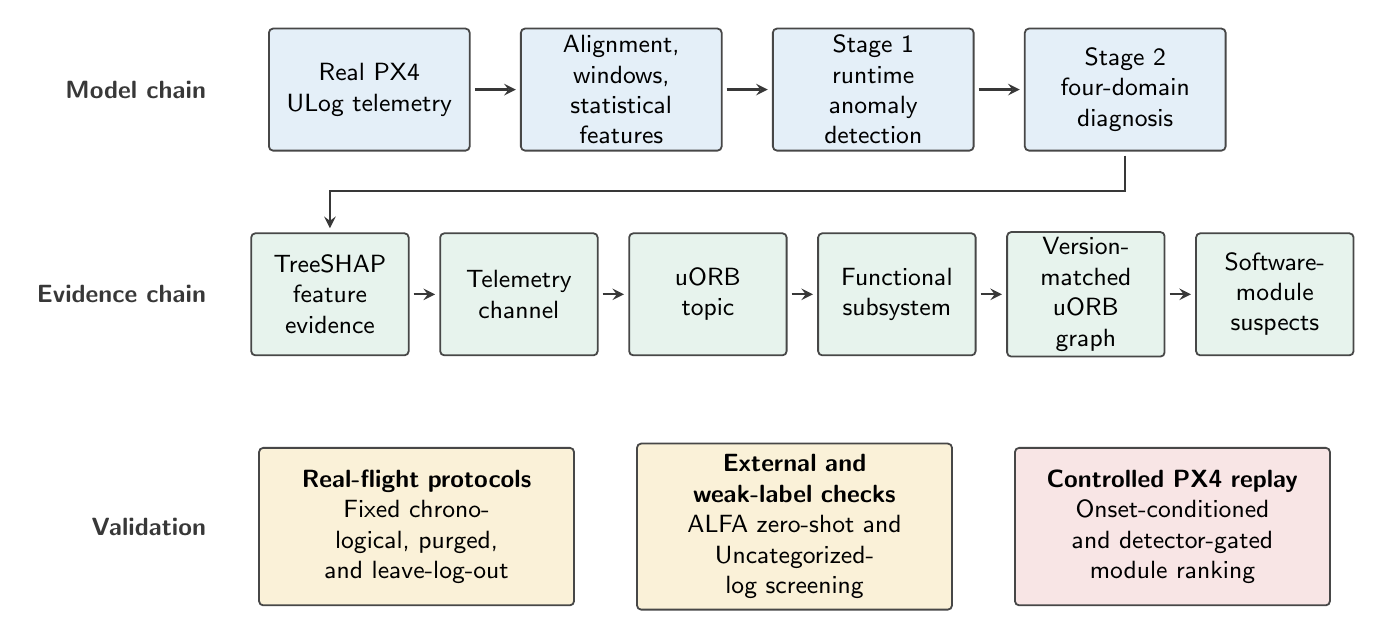
\begin{tikzpicture}[
    font=\sffamily\small,
    block/.style={draw=black!72, rounded corners=1.5pt, line width=0.65pt, align=center, minimum width=2.55cm, minimum height=1.55cm, text width=2.15cm, inner sep=2pt},
    evidence/.style={draw=black!72, rounded corners=1.5pt, line width=0.65pt, align=center, minimum width=2.00cm, minimum height=1.55cm, text width=1.70cm, inner sep=2pt},
    validation/.style={draw=black!72, rounded corners=1.5pt, line width=0.65pt, align=center, minimum width=4.00cm, minimum height=2.00cm, text width=3.55cm, inner sep=4pt},
    flow/.style={->, draw=black!78, line width=0.85pt, >=stealth, shorten <=1.5pt, shorten >=1.5pt},
    rowlabel/.style={anchor=east, font=\sffamily\bfseries\small, text=black!78}
]
\definecolor{modelblue}{RGB}{228,239,248}
\definecolor{evidencegreen}{RGB}{231,243,237}
\definecolor{validationgold}{RGB}{250,241,216}
\definecolor{boundaryred}{RGB}{248,229,229}

\node[rowlabel] at (-0.15,4.70) {Model chain};
\node[block, fill=modelblue] (ulog) at (1.80,4.70) {Real PX4\\ULog telemetry};
\node[block, fill=modelblue] (features) at (5.00,4.70) {Alignment, windows,\\statistical features};
\node[block, fill=modelblue] (stage1) at (8.20,4.70) {Stage 1\\runtime anomaly\\detection};
\node[block, fill=modelblue] (stage2) at (11.40,4.70) {Stage 2\\four-domain\\diagnosis};
\draw[flow] (ulog) -- (features);
\draw[flow] (features) -- (stage1);
\draw[flow] (stage1) -- (stage2);

\node[rowlabel] at (-0.15,2.10) {Evidence chain};
\node[evidence, fill=evidencegreen] (shap) at (1.30,2.10) {TreeSHAP\\feature\\evidence};
\node[evidence, fill=evidencegreen] (channel) at (3.70,2.10) {Telemetry\\channel};
\node[evidence, fill=evidencegreen] (topic) at (6.10,2.10) {uORB\\topic};
\node[evidence, fill=evidencegreen] (subsystem) at (8.50,2.10) {Functional\\subsystem};
\node[evidence, fill=evidencegreen] (graph) at (10.90,2.10) {Version-matched\\uORB graph};
\node[evidence, fill=evidencegreen] (suspects) at (13.30,2.10) {Software-module\\suspects};
\draw[flow] (shap) -- (channel);
\draw[flow] (channel) -- (topic);
\draw[flow] (topic) -- (subsystem);
\draw[flow] (subsystem) -- (graph);
\draw[flow] (graph) -- (suspects);
\draw[flow] (stage2.south) -- ++(0,-0.50) -| (shap.north);

\node[rowlabel] at (-0.15,-0.85) {Validation};
\node[validation, fill=validationgold] (internal) at (2.40,-0.85) {\textbf{Real-flight protocols}\\Fixed chronological, purged,\\and leave-log-out};
\node[validation, fill=validationgold] (external) at (7.20,-0.85) {\textbf{External and weak-label checks}\\ALFA zero-shot and\\Uncategorized-log screening};
\node[validation, fill=boundaryred] (replay) at (12.00,-0.85) {\textbf{Controlled PX4 replay}\\Onset-conditioned and detector-gated\\module ranking};
\end{tikzpicture}
}
    \caption{Overview of HS-AeroTS. The model chain performs runtime anomaly detection followed by four-domain diagnosis. TreeSHAP evidence is aggregated from statistical features to telemetry channels, uORB topics, and subsystems, and a static uORB graph reconstructed at the selected majority firmware commit produces software-module suspects. Three validation branches separately test real-flight robustness, external or weak-label transfer, and controlled replay under onset-conditioned and detector-gated protocols.}
    \label{fig:framework_overview}
\end{figure}

\begin{table}[H]
\caption{Research questions, corresponding experiments, primary metrics, and evidence levels.\label{tab:research_questions}}
\footnotesize
\begin{tabularx}{\textwidth}{>{\raggedright\arraybackslash}p{0.65cm} >{\raggedright\arraybackslash}p{5.00cm} >{\raggedright\arraybackslash}p{3.15cm} >{\raggedright\arraybackslash}X}
\toprule
\textbf{RQ} & \textbf{Corresponding experiments} & \textbf{Primary metrics} & \textbf{Evidence level}\\
\midrule
RQ1 & Runtime anomaly detection and four-domain diagnosis under fixed chronological, purged, leave-log-out, ALFA zero-shot, and Uncategorized-log protocols & AUPRC, AUROC, Macro-F1, Balanced Accuracy, per-class Recall & Runtime anomaly and fault-domain evidence; no source-code ground truth\\
RQ2 & SHAP conservation, top-$k$ masking versus random masking, Consistency@$K$/Hit@$K$, and majority-commit topic--module mapping & Conservation error, Macro-F1 decrease, Consistency@$K$, Hit@$K$, mapping coverage and firmware-version coverage & Feature, channel, topic, subsystem, and static architecture-association evidence\\
RQ3 & Controlled PX4 ULog replay with known source mutations; onset-conditioned and detector-gated evaluation & Detector recall, Top-1/3/5, MRR, EXAM & Mutation-ground-truth ranking evidence, explicitly conditioned on the evaluation gate\\
\bottomrule
\end{tabularx}
\end{table}
